\subsection{Git (Magnus)}

Gruppen har ofte mødtes fysisk. Typisk har disse møder fulgt formatet:

\begin{enumerate}
\item \textbf{Læs logbog:} Få overblik over hvad der skete sidst, ved brug af logbog og commit messages.
\item \textbf{Opdel} dagens opgaver, fx “Skriv tests i Employee klassen”.
\item \textbf{Branch} i Git. Gerne i 2 grupper af 2 personer, så hver koder har en idé- og sparringspartner, eller i 4 énmandsgrupper, så der kan blive implementeret fx mange tests på én gang uden filkonflikter.
\item \textbf{Implementér} de udvalgte opgaver i grupperne.
\item \textbf{Merge} branches, løs eventuelle mergekonflikter.
\item \textbf{Skriv logbog:} Opdatér logbogen med hensyn til dagens arbejde, og fremtidigt fokus.
\end{enumerate}


Der blev skrevet og implementeret mange tests og features, hvilket klart blev gjort lettere med Git. Eksempelvis kunne én person skrive en test (branch $\rightarrow$ skriv JUnit test $\rightarrow$ merge), hvorefter en anden kunne implementere den (branch $\rightarrow$ implementér løsning i fx Employee.java $\rightarrow$ merge). 
 

\begin{figure}[H]
    \centering
    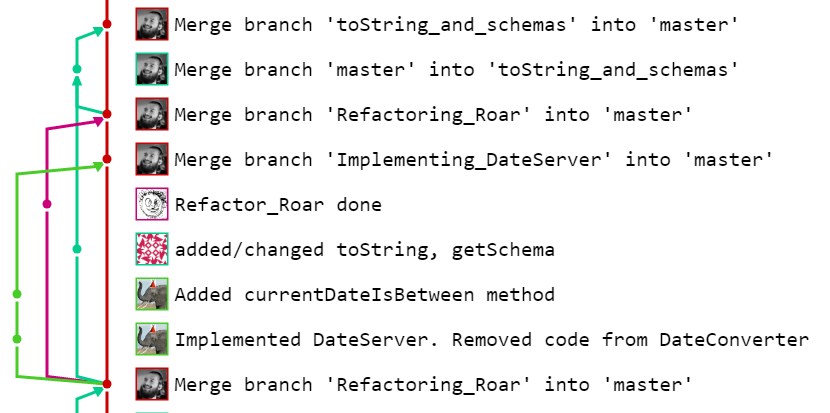
\includegraphics[width = 0.8\textwidth]{Figurer/git_branches.PNG}
    \caption{Branching og merging ved et fysisk møde, hvor gruppen fokuserede på programmets håndtering af datoer og toString metoder.}
    \label{fig:gitex}
\end{figure}

